% Options for packages loaded elsewhere
\PassOptionsToPackage{unicode}{hyperref}
\PassOptionsToPackage{hyphens}{url}
\PassOptionsToPackage{dvipsnames,svgnames,x11names}{xcolor}
%
\documentclass[
  11pt,
]{article}

\usepackage{amsmath,amssymb}
\usepackage{iftex}
\ifPDFTeX
  \usepackage[T1]{fontenc}
  \usepackage[utf8]{inputenc}
  \usepackage{textcomp} % provide euro and other symbols
\else % if luatex or xetex
  \usepackage{unicode-math}
  \defaultfontfeatures{Scale=MatchLowercase}
  \defaultfontfeatures[\rmfamily]{Ligatures=TeX,Scale=1}
\fi
\usepackage{lmodern}
\ifPDFTeX\else  
    % xetex/luatex font selection
    \setmainfont[]{Aptos}
\fi
% Use upquote if available, for straight quotes in verbatim environments
\IfFileExists{upquote.sty}{\usepackage{upquote}}{}
\IfFileExists{microtype.sty}{% use microtype if available
  \usepackage[]{microtype}
  \UseMicrotypeSet[protrusion]{basicmath} % disable protrusion for tt fonts
}{}
\makeatletter
\@ifundefined{KOMAClassName}{% if non-KOMA class
  \IfFileExists{parskip.sty}{%
    \usepackage{parskip}
  }{% else
    \setlength{\parindent}{0pt}
    \setlength{\parskip}{6pt plus 2pt minus 1pt}}
}{% if KOMA class
  \KOMAoptions{parskip=half}}
\makeatother
\usepackage{xcolor}
\setlength{\emergencystretch}{3em} % prevent overfull lines
\setcounter{secnumdepth}{-\maxdimen} % remove section numbering
% Make \paragraph and \subparagraph free-standing
\makeatletter
\ifx\paragraph\undefined\else
  \let\oldparagraph\paragraph
  \renewcommand{\paragraph}{
    \@ifstar
      \xxxParagraphStar
      \xxxParagraphNoStar
  }
  \newcommand{\xxxParagraphStar}[1]{\oldparagraph*{#1}\mbox{}}
  \newcommand{\xxxParagraphNoStar}[1]{\oldparagraph{#1}\mbox{}}
\fi
\ifx\subparagraph\undefined\else
  \let\oldsubparagraph\subparagraph
  \renewcommand{\subparagraph}{
    \@ifstar
      \xxxSubParagraphStar
      \xxxSubParagraphNoStar
  }
  \newcommand{\xxxSubParagraphStar}[1]{\oldsubparagraph*{#1}\mbox{}}
  \newcommand{\xxxSubParagraphNoStar}[1]{\oldsubparagraph{#1}\mbox{}}
\fi
\makeatother


\providecommand{\tightlist}{%
  \setlength{\itemsep}{0pt}\setlength{\parskip}{0pt}}\usepackage{longtable,booktabs,array}
\usepackage{calc} % for calculating minipage widths
% Correct order of tables after \paragraph or \subparagraph
\usepackage{etoolbox}
\makeatletter
\patchcmd\longtable{\par}{\if@noskipsec\mbox{}\fi\par}{}{}
\makeatother
% Allow footnotes in longtable head/foot
\IfFileExists{footnotehyper.sty}{\usepackage{footnotehyper}}{\usepackage{footnote}}
\makesavenoteenv{longtable}
\usepackage{graphicx}
\makeatletter
\def\maxwidth{\ifdim\Gin@nat@width>\linewidth\linewidth\else\Gin@nat@width\fi}
\def\maxheight{\ifdim\Gin@nat@height>\textheight\textheight\else\Gin@nat@height\fi}
\makeatother
% Scale images if necessary, so that they will not overflow the page
% margins by default, and it is still possible to overwrite the defaults
% using explicit options in \includegraphics[width, height, ...]{}
\setkeys{Gin}{width=\maxwidth,height=\maxheight,keepaspectratio}
% Set default figure placement to htbp
\makeatletter
\def\fps@figure{htbp}
\makeatother

\usepackage{booktabs}
\usepackage{longtable}
\usepackage{array}
\usepackage{multirow}
\usepackage{wrapfig}
\usepackage{float}
\usepackage{colortbl}
\usepackage{pdflscape}
\usepackage{tabu}
\usepackage{threeparttable}
\usepackage{threeparttablex}
\usepackage[normalem]{ulem}
\usepackage{makecell}
\usepackage{xcolor}
\usepackage{pdfpages}
\usepackage{fontspec}
\usepackage[bottom]{footmisc}
\setmainfont{Aptos}[Path="C:/Users/ginow/AppData/Roaming/TinyTeX/texmf-dist/fonts/truetype/aptos/", Extension=".ttf"]
\usepackage{fancyhdr}
\pagestyle{fancy}
\fancyhf{}
\fancyhead[C]{\makebox[\textwidth]{\hspace*{-1cm}
\includegraphics[height=1.9cm]{../Logotipo ENADEL/encabezado_izquierda.png} \hfill 
\includegraphics[height=1.5cm]{../Logotipo ENADEL/encabezado_derecha.png} \hspace*{-2cm}}}
\fancyfoot[L]{Subsecretaría del Trabajo}
\cfoot{\thepage}
\setlength{\footskip}{10pt}
\setlength{\skip\footins}{15pt}
\setlength{\headheight}{3cm}
\setlength{\headsep}{0.5cm}
\renewcommand{\footrulewidth}{0pt}
\floatplacement{figure}{H}
\floatplacement{table}{H}
\usepackage{geometry}
\geometry{ left=3cm, right=3cm, top=2.5cm, bottom=2.5cm }
\usepackage{placeins}
\usepackage{ragged2e}
\usepackage{float}
\usepackage{setspace}
\renewcommand{\familydefault}{\sfdefault}
\AtBeginDocument{\renewcommand{\baselinestretch}{1.5}\justifying}
\usepackage{xcolor}
\usepackage{pagecolor}
\makeatletter
\@ifpackageloaded{caption}{}{\usepackage{caption}}
\AtBeginDocument{%
\ifdefined\contentsname
  \renewcommand*\contentsname{Tabla de contenidos}
\else
  \newcommand\contentsname{Tabla de contenidos}
\fi
\ifdefined\listfigurename
  \renewcommand*\listfigurename{Listado de Figuras}
\else
  \newcommand\listfigurename{Listado de Figuras}
\fi
\ifdefined\listtablename
  \renewcommand*\listtablename{Listado de Tablas}
\else
  \newcommand\listtablename{Listado de Tablas}
\fi
\ifdefined\figurename
  \renewcommand*\figurename{Figura}
\else
  \newcommand\figurename{Figura}
\fi
\ifdefined\tablename
  \renewcommand*\tablename{Tabla}
\else
  \newcommand\tablename{Tabla}
\fi
}
\@ifpackageloaded{float}{}{\usepackage{float}}
\floatstyle{ruled}
\@ifundefined{c@chapter}{\newfloat{codelisting}{h}{lop}}{\newfloat{codelisting}{h}{lop}[chapter]}
\floatname{codelisting}{Listado}
\newcommand*\listoflistings{\listof{codelisting}{Listado de Listados}}
\makeatother
\makeatletter
\makeatother
\makeatletter
\@ifpackageloaded{caption}{}{\usepackage{caption}}
\@ifpackageloaded{subcaption}{}{\usepackage{subcaption}}
\makeatother

\ifLuaTeX
\usepackage[bidi=basic]{babel}
\else
\usepackage[bidi=default]{babel}
\fi
\babelprovide[main,import]{spanish}
\ifPDFTeX
\else
\babelfont{rm}[]{Aptos}
\fi
% get rid of language-specific shorthands (see #6817):
\let\LanguageShortHands\languageshorthands
\def\languageshorthands#1{}
\ifLuaTeX
  \usepackage{selnolig}  % disable illegal ligatures
\fi
\usepackage{bookmark}

\IfFileExists{xurl.sty}{\usepackage{xurl}}{} % add URL line breaks if available
\urlstyle{same} % disable monospaced font for URLs
\hypersetup{
  pdflang={es},
  colorlinks=true,
  linkcolor={blue},
  filecolor={Maroon},
  citecolor={Blue},
  urlcolor={Blue},
  pdfcreator={LaTeX via pandoc}}


\author{}
\date{}

\begin{document}


\includepdf[pages=-]{../Quarto/Portada/Portada_ENADEL 2024.pdf}


\definecolor{customblue}{HTML}{005691}

\pagecolor{customblue} 
\thispagestyle{empty} 
\color{white}

\centering


\includegraphics[width=0.5\textwidth]{../Logotipo ENADEL/Logotipo ENADEL-02.png}
\vspace{2cm}

\noindent Ministerio del Trabajo y Previsión Social

División de Políticas de Empleo\textbackslash{} Subsecretaría del
Trabajo

\justifying

El presente documento analiza los resultados de la Encuesta Nacional de
Demanda Laboral (ENADEL) 2024, que busca identificar y caracterizar el
capital humano requerido por las empresas de los distintos sectores
productivos del país, generando información sobre la demanda actual de
ocupaciones de las empresas, detectando requisitos y problemas de
contratación. A diferencia de las versiones anteriores de esta encuesta,
la actual versión abarca 15 sectores de actividad económica, ayuda a
identificar prioridades de capacitación y se añade el foco sobre el
impacto que está teniendo la incorporación de nuevas tecnologías y los
eventos climáticos extremos sobre los trabajadores.

\newpage
\nopagecolor
\color{black}
\renewcommand{\contentsname}{Índice} 
\tableofcontents

\newpage

\subsection{Capítulo I: Contexto y caracterización de
empresas}\label{capuxedtulo-i-contexto-y-caracterizaciuxf3n-de-empresas}

\subsubsection{Producto/Servicio}\label{productoservicio}

\FloatBarrier

\subsubsection{Regiones y ubicación de
sucursales}\label{regiones-y-ubicaciuxf3n-de-sucursales}

La muestra de ENADEL 2024 encuesta a 6.490 empresas que suman 485.256
trabajadores (a nivel muestral). Estas representan a 82.052 empresas y
5.611.196 trabajadores a nivel nacional. La Tabla~\ref{tbl-region}
muestra la distribución en las distintas regiones del país, dónde un
\text{8}\% de las empresas y un \text{16,1}\% de los trabajadores se
encuentran en la región Metropolitana.

\vspace{5mm}

\FloatBarrier

\begin{table}

\caption{\label{tbl-region}Resultados de la encuesta}

\centering{

\centering
\begin{tabular}{>{\raggedright\arraybackslash}p{6cm}>{\raggedright\arraybackslash}p{3cm}>{\raggedright\arraybackslash}p{3cm}}
\toprule
Región & \% Empresas & \% Trabajadores\\
\midrule
Arica y Parinacota & 4\% & 0,3\%\\
Tarapacá & 6\% & 7,2\%\\
Antofagasta & 4\% & 27,8\%\\
Atacama & 8\% & 1,9\%\\
Coquimbo & 2\% & 0,3\%\\
\addlinespace
Valparaíso & NA\% & NA\%\\
Metropolitana & 8\% & 16,1\%\\
O'Higgins & 6\% & 5\%\\
Maule & 12\% & 3,9\%\\
Ñuble & 16\% & 2,7\%\\
\addlinespace
Biobío & 10\% & 19,1\%\\
Araucanía & 2\% & 0,2\%\\
Los Ríos & 14\% & 10,8\%\\
Los Lagos & 2\% & 0,1\%\\
Aysén & 2\% & 2,7\%\\
\addlinespace
Magallanes & 4\% & 2,1\%\\
\bottomrule
\multicolumn{3}{l}{\rule{0pt}{1em}Fuente: Elaboración propia utilizando datos de ENADEL 2024, datos expandidos.}\\
\end{tabular}

}

\end{table}%

La Figura~\ref{fig-mapa-sucursal} ilustra las regiones donde las
empresas tienen sucursales, las regiones con más cantidad de sucursales
que corresponden a sedes no principales son Los Ríos, Libertador General
Bernardo O'Higgins y Maule con un total de 17, 11 y 11 sucursales
respectivamente. Por su parte, las regiones de Aisén del General Carlos
Ibáñez del Campo, Magallanes y Antártica Chilena y Valparaíso registran
la menor presencia de sucursales regionales de las empresas, con 3 o
menos dependencias.

\FloatBarrier

\begin{figure}[H]

\caption{\label{fig-mapa-sucursal}Sucursales por región}

\centering{

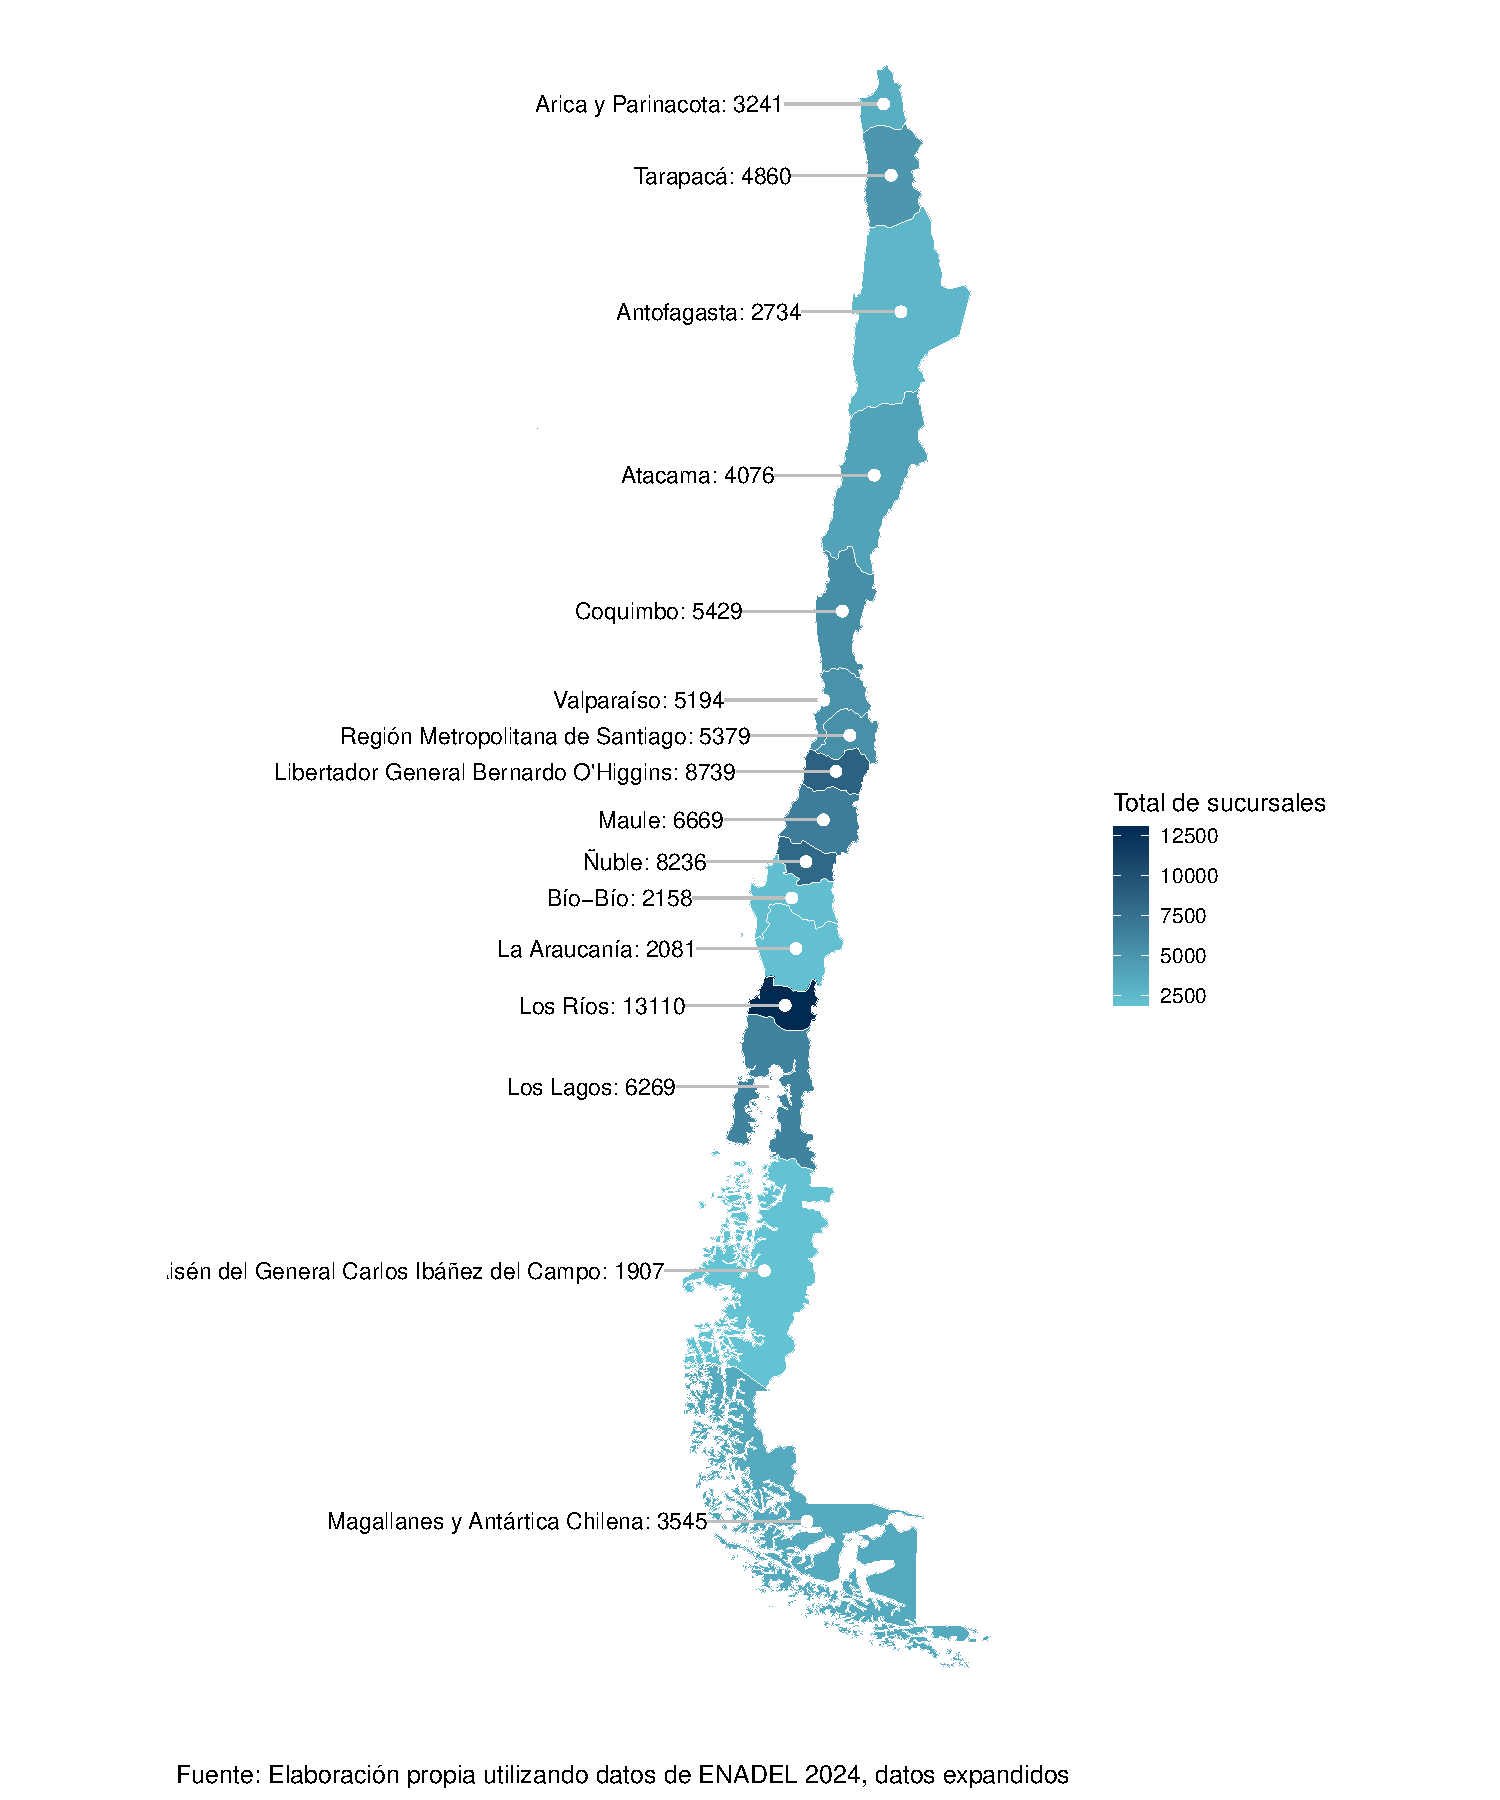
\includegraphics{reporte_2024_files/figure-pdf/fig-mapa-sucursal-1.pdf}

}

\end{figure}%

\FloatBarrier

\subsubsection{Tamaño de empresas (n° de ventas y n° de
trabajadores)}\label{tamauxf1o-de-empresas-n-de-ventas-y-n-de-trabajadores}

La Figura~\ref{fig-combined} muestra el porcentaje de empresas y
trabajadores según tamaño de empresas, utilizando la clasificación por
número de trabajadores, cómo por volumen de venta. Con respecto a la
primera clasificación, el 74,6\% de las empresas tiene menos de 50
trabajadores --acumulando un 23,8\% del total-- y casi el 50\% de los
trabajadores están en empresas grandes --que corresponden a un 6,5\% del
total. Si se analiza según tamaño de ventas, más de la mitad de las
empresas tienen un volumen de venta de entre 2.400 y 24.999 UF
(``Pequeñas'') y más de un cuarto venden entre 25.000 y 100.000 UF al
año (``Mediana''). Sin embargo, casi un tercio de los trabajadores están
en empresas grandes (más de 100.000 UF).

\FloatBarrier

\begin{figure}[H]

\caption{\label{fig-combined}Gráfico combinado de resultados}

\centering{

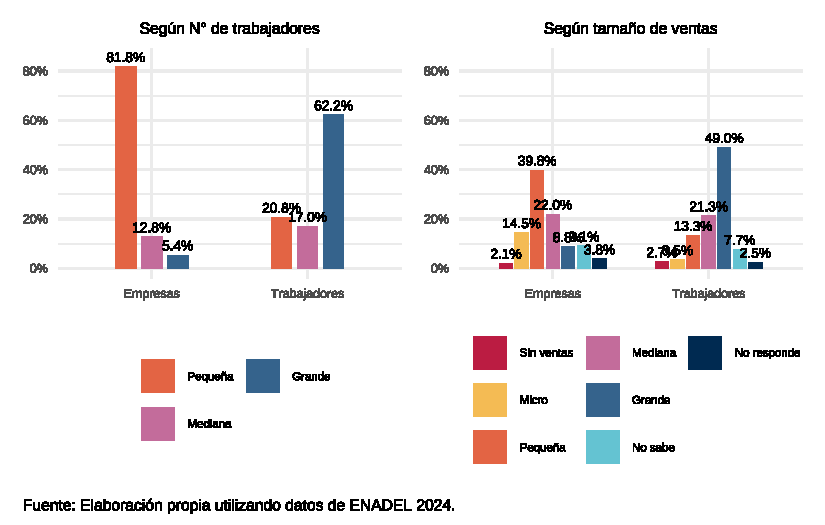
\includegraphics[width=1\textwidth,height=\textheight]{reporte_2024_files/figure-pdf/fig-combined-1.pdf}

}

\end{figure}%

\FloatBarrier

Al revisar la distribución por sector de actividad económica
Tabla~\ref{tbl-acteco} se tiene que una de cada cinco empresas pertenece
al sector de Comercio, seguido por el sector Construcción (\text{7,6}\%)
y el sector de Industrias Manufactureras (11,4\%). Con respecto al
volumen de trabajadores, el sector Comercio también lidera (17,8\%)
seguido por el sector Construcción (14,4\%) y el sector de Servicios
Administrativos y de Apoyo que, siendo sector intensivo en trabajo, un
9,1\% de las empresas acumula el 13,5\% de trabajadores y trabajadoras.

\FloatBarrier

\begin{table}

\caption{\label{tbl-acteco}Empresas y trabajadores según sector de
actividad económica}

\centering{

\centering
\begin{tabular}{>{\raggedright\arraybackslash}p{11cm}ll}
\toprule
Actividad Económica & \% Empresas & \% Trabajadores\\
\midrule
Agricultura, ganadería, silvicultura y pesca & 14,3\% & 18,7\%\\
Industrias manufactureras & 7,6\% & 17,3\%\\
Suministro de electricidad, gas, agua  y gestión de desechos & 11,3\% & 15\%\\
Construcción & 20,7\% & 14,5\%\\
Comercio & 9\% & 9,8\%\\
\addlinespace
Transporte y almacenamiento & 15,9\% & 7,2\%\\
Alojamiento y de servicio de comidas & 4,8\% & 7,2\%\\
Información y comunicaciones & 4,1\% & 3,3\%\\
Actividades financieras y de seguros & 3,4\% & 2,3\%\\
Actividades inmobiliarias & 3\% & 2,2\%\\
\addlinespace
Actividades profesionales, científicas y de servicios administrativos & 5,3\% & 2,2\%\\
Actividades artísticas, de entretenimiento y otros servicios & 0,7\% & 0,4\%\\
\bottomrule
\multicolumn{3}{l}{\rule{0pt}{1em}Fuente: Elaboración propia utilizando datos de ENADEL 2024, datos expandidos.}\\
\end{tabular}

}

\end{table}%

\FloatBarrier

\subsubsection{Estructura corporativa
(conglomerado/subcontrato)}\label{estructura-corporativa-conglomeradosubcontrato}

\subsection{Capítulo II: Demanda Laboral y Ocupaciones de Difícil
Cobertura}\label{capuxedtulo-ii-demanda-laboral-y-ocupaciones-de-difuxedcil-cobertura}

\subsubsection{Demanda Laboral}\label{demanda-laboral}

\subsubsection{Contrataciones}\label{contrataciones}

\subsubsection{Ocupaciones}\label{ocupaciones}

\subsubsection{Ocupaciones de Difícil
Cobertura}\label{ocupaciones-de-difuxedcil-cobertura}

\subsubsection{Principales Dificultades}\label{principales-dificultades}

\subsubsection{Resultado de Movilidad}\label{resultado-de-movilidad}

\subsection{Capítulo III: Capacitación y
Habilidades}\label{capuxedtulo-iii-capacitaciuxf3n-y-habilidades}

\subsubsection{Organismo Técnico Intermedio para
capacitación}\label{organismo-tuxe9cnico-intermedio-para-capacitaciuxf3n}

\subsubsection{Capacitaciones de la
empresa}\label{capacitaciones-de-la-empresa}

\subsubsection{Competencias en que se
capacita}\label{competencias-en-que-se-capacita}

\subsubsection{Fuentes de financiamiento de la
capacitación}\label{fuentes-de-financiamiento-de-la-capacitaciuxf3n}

\subsection{Capítulo IV:
Transiciones}\label{capuxedtulo-iv-transiciones}

\subsubsection{Eventos climáticos
extremos}\label{eventos-climuxe1ticos-extremos}

\subsubsection{Medidas de Cuidado del
medioambiente}\label{medidas-de-cuidado-del-medioambiente}

\subsubsection{Digitalización y
Automatización}\label{digitalizaciuxf3n-y-automatizaciuxf3n}

\paragraph{Cambios en dotación de
personal}\label{cambios-en-dotaciuxf3n-de-personal}

\paragraph{Creación de nuevos puestos de
trabajo}\label{creaciuxf3n-de-nuevos-puestos-de-trabajo}

\paragraph{Dificultad para llenar
vacantes}\label{dificultad-para-llenar-vacantes}




\end{document}
